\section{Using computational models for Biological Analysis}
\epigraph{The following chapter was written by members of the University of Miami }{\textit{iGEM MiamiU\_OH 2021}}
\noindent
MATLAB and Python are powerful programs that can be used to manipulate matrices and perform complicated numerical analysis. In the case of synthetic biology, these environments are often used to set up models for biological action, or mathematical representations of complex systems. These mathematical representations can extend to systems with multiple enzymes and interconnected reactions, like the metabolism within the cell. Therefore, through platforms such as MATLAB and Python, we can generate a complex system of inputs and outputs that interact with each other to generate a projection modeling the activity of a system representing a multitude of cells, a single cell, or a microenvironment within a cell. The origin for this method of thinking can be traced back to Boolean circuits, a common mathematical method for combining logic circuits in digital electronic circuits. While these Boolean circuits are useful for projecting basic biological loops, they are not effective to model something as complex as an entire cell through virtual circuits. Instead, a model based on a more complex system of mathematical equations must be used. Dry lab tests using these models allow the team to assess proposed systems or predict outcomes prior to commitment of physical and temporal resources in the wet lab.\\
Although models can be applied to a host of scientific inquiries, due to a primary focus in synthetic and systems biology for phototrophs on using and understanding their metabolic features, this chapter will focus on the analysis of an organism’s metabolism \parencite{Klemencic2017}.

\subsection{COBRA (Constraint-Based Reconstruction and Analysis Toolbox)}
To enable teams to test the impacts of these proposed conditions or added networks on both metabolic reaction fluxes, or rates, and growth of the cells in a dry lab setting, multiple software can be used. However, in this chapter, we will focus on the widely used \href{https://opencobra.github.io/cobratoolbox/stable/index.html}{Constraint-Based Reconstruction and Analysis Toolbox (COBRA)}. A constraint-based model for biochemical networks has a wide range of uses. In the case of analyzing the metabolism of cells, we can input a set of metabolites, reactions, enzymes, kinetic data, and/or stoichiometric coefficients into matrices that are readable by the COBRA Toolbox. Then we input specific constraints to how these inputs can interact that reflect biological limits or desired conditions. From this common set of inputs and constraints, the COBRA Toolbox can present a field of permissible outcomes, in our case fluxes of the different reactions, that allow optimization of a certain condition. This means our team could utilize the toolbox in both MATLAB and Python to generate a host of flux outcomes for any system, or cell with clarified available reaction pathways, that would allow optimization in an area such as production of a metabolite or in growth. This analysis simplifies the temporal and informational demands for the design team as well as provides valuable insight into the feasibility and wet lab parameters for proposed pathways or conditions.

\subsection{Kinetics vs Flux Based Models}
The cell operates via the action of a myriad of enzymatic systems and interactions. From a simple material balance standpoint, mass must be conserved. Our overall system is the cell, and the agents of action are reaction cascades. Within this cell/system, the reaction cascades are observed, and the operators of those cascades are individual enzymatic reactions (4). For these reactions, we have multiple considerations to potentially consider, including thermodynamics, metabolites, enzyme kinetics, mass balances, and enzymatic capacity. All of these are \textit{constraints}, and a model could be defined from a combination of these constraints \parencite{Yasemi2021}.  \\ \\
Reactions are primarily limited by enzymatic kinetics (“speed”) and flux (turnovers of metabolites). Therefore, most models are based on either of these two constraints. Kinetics based models are based on differential equations relating the rates of reactions, taking both kinetics and genetic-based regulation into account. Unfortunately, this model requires enzymatic kinetic data specific to the organism of interest, most of which is unavailable and therefore must be estimated; this guesswork introduces significant source for potential error \parencite{Yasemi2021}. Conversely, flux-based models use stoichiometric information of all reactions as their constraints, and therefore circumvent the need for kinetic data \parencite{Orth2010}. This model, however, does not take kinetics or genetic regulation into account and therefore is not as robust in analysis as kinetics-based models. Still, it finds the fluxes of metabolites through the defined metabolic network, allowing calculations of growth and productions of metabolites of interest. Due to the availability of a significantly validated flux-based model for our strain of interest, we chose to work with a flux-based model. 


\subsection{Mathematical Justification of a Flux-based Model using FBA}
Let’s go through a simple flux-based model simulating a cell, or metabolic network, with three metabolites: $A, B$, and $C$ connected by the reaction $A\rightarrow B+C$. 
We can represent the flux of $A\rightarrow B$ and $A\rightarrow C$ with the flux values, $v_1$ for $A$, $v_2$ for $B$, and $v_3$ for $C$. If we go further and state that the relationship includes assigned stoichiometric coefficients, $c_1$, $c_2$, and $c_3$ for metabolites $A$, $B$, and $C$ respectively, we get the following expression:
$$\Psi(v) = c_1v_1 + c_2v_2 + c_3v_3$$
This is a valid statement so long as conservation of mass holds true, where the input flux and output flux are represented by $v_i$ and $v_o$:
$$v_i=v_o$$
While mass needs to be conserved, the direction of the reaction is not fixed unless we specify it as such. Holding  positive makes the reaction progress forward and making  negative reverses the reaction. We can use a stoichiometric matrix for the reaction to define the flux relationship such that:
$$\left(c_1 c_2  c_3\right)  \times \left(v_1 v_2  v_3\right) = \Psi(v)= (0 0 0) $$
Each row corresponds to the assigned metabolite, $A$, $B$, and $C$. $\Psi$ is expressed as equaling $0$ because the primary assumption on which flux-based analysis is made is a steady state condition. Steady state describes a system that is not experiencing internal change even if the inputs and outputs are different from each other. In other words, the net concentration of a metabolite is constant), or the net flux of the reaction is $0$, based on the overall processes (or reactions), inputting and outputting the species balancing each other out. It’s important to clarify that the fluxes of the individual reactions involved with this metabolite are not necessarily $0$, but instead the combination of all these reactions allows the net flux of this metabolite to be 0. This equation summarizes the objective function for one reaction, but we can now expand on this to represent multiple reactions. To model an entire cell, that will be necessary.  The matrix with coefficients is referred to as the S-matrix, and this S-matrix can hold more columns that correspond to infinitely many reactions. 
$$\Psi(v)=c_1v_1 + c_2v_2+(\ldots)+c_nv_n$$
$$
\left(c_{11} c_{12} c_{13} c_{14} \ldots c_{21} c_{22} c_{23} c_{24} \ldots c_{31} c_{32} c_{33} c_{34} \ldots\right) \times \left( v_1 v_2 v_3 \ldots\right)  = \Psi(v)=\left(0 0 0 \right)  $$
The number of terms in the flux equation is determined by the number of reactions occurring in the model. Now, we can specify a reaction to each column of the $S$-matrix given the relationship between upper and lower bounds, or limits, of the reaction set:
$$lb_n<v_n<ub_n$$
\noindent
Using linear programming based on all these metabolic constraints as well as any additional desired constraints, $\Psi(v)$ can be optimized. With defined $c$ values, constricted ranges for $v$, or fluxes, the steady state assumption, and any other provided constraints, the fluxes of the reactions that allow the optimized solution can be solved. Computational linear programming algorithms such as the COBRA Toolbox are used to solve these equations.

\section{Building a Model}
\subsection{Adding Reactions and Metabolites}
Flux-based models are based on a set of reactions, metabolites, and the stoichiometric matrices of these metabolites in each reaction. Optional additions include gene-protein-reaction assignments where genes with proper locus tags according to available genomes of an organism are assigned to reactions. For finding the proper reactions, suggested metabolite names, and expected genes corresponding to said reactions, the Kyoto Encyclopedia of Genes and Genomes (KEGG) is highly recommended and can be found \href{https://www.kegg.jp/}{here}. KEGG is a large database that holds multiple pathways, genomes, metabolites, reactions, enzyme nomenclature, and maps of these reactions for general processes as well as those specific to an organism of interest. This is not all that KEGG does, but the immediate application for validated data is obvious when it comes to model development.
\begin{enumerate}
    \item  One should consider all of the reactions that should be included in this model. It should be noted that not incorporating key reactions can severely undermine the model’s results. Therefore, the model should at bare minimum not only include the reactions of interest, but all reactions involved in central metabolism and those expected to have some kind of implication on your pathway of interest. Once the reactions are determined, you must create variables for all of the metabolites involved in these reactions. As an example, I can want to add the simple reaction of PEP carboxylase which carboxylates phosphoenolpyruvate to become oxaloacetate. According to KEGG, the reaction is “phosphoenol pyruvate + 2 bicarbonates <-> oxaloacetate.”
    \item First, one needs to create variables for each of the metabolites. It is suggested to create an excel sheet with the full name of the metabolite followed by a metabolic\_id that can be accessed by the model. In other words, the metabolic\_id is a shortened version that means you don’t have to write insanely long chemical names all the time. In the case of the metabolites above I choose pep\_c for phosphoenol pyruvate, hco3\_c for bicarbonate, and oaa\_c for oxaloacetate.
    \item Then I need to create a stoichiometric matrix that combines the reactions with the metabolites. Each row will be a different metabolite and the column will correspond to a different reaction. The numbers correspond to the number of moles of that metabolite being used (negative) or produced (positive) in that reaction. In the case of my reaction, it would look like the following:
\begin{table}[!htpb]
\centering
\begin{tabular}{|l|l|} 
\hline
        & R1  \\ 
\hline
pep\_c  & -1  \\
hco3\_c & -2  \\
oaa\_c  & 1   \\
\hline
\end{tabular}
\end{table}
\FloatBarrier

    \item Ultimately, a list of these can be made by forming a massive matrix. A template by which one can follow for a pathway is shown below.
    
    \begin{figure}[!htbp]
    \centering
    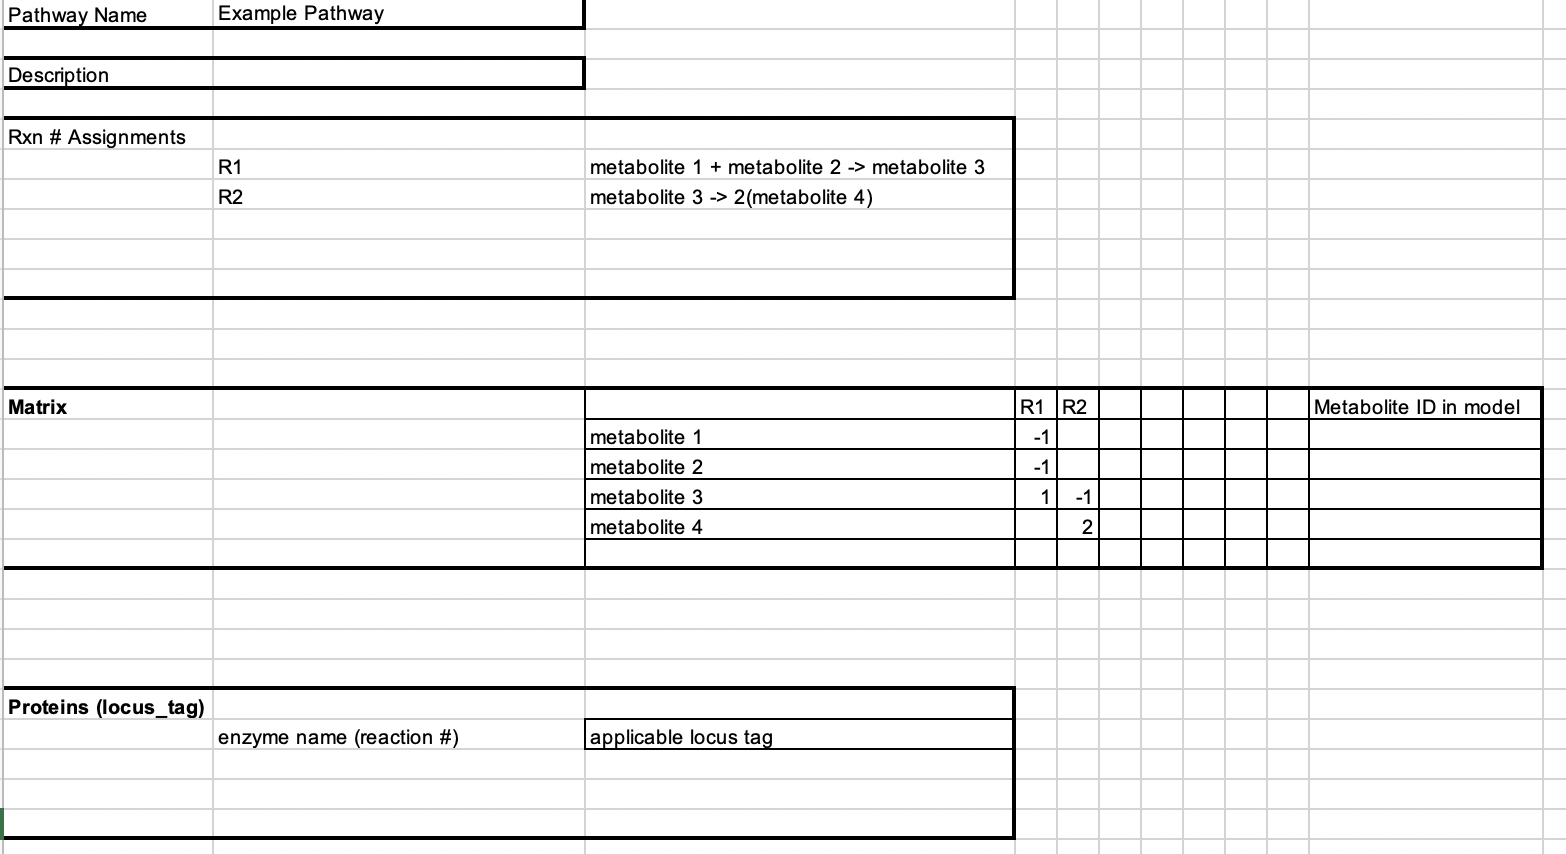
\includegraphics[width=0.7\textwidth]{images/chap8/image01.png}
    \label{fig:ch801}
    \end{figure}
    \FloatBarrier

    \item These can then be added to the model using functions found for matlab \href{https://opencobra.github.io/cobratoolbox/stable/modules/analysis/FBA/index.html}{here} under flux balanced analysis or for python \href{https://cobrapy.readthedocs.io/en/latest/}{here}. 
\end{enumerate}

\subsection{Creating an Objective}
One needs to create an objective for which the model can solve. This is most likely biomass production or a reaction. If it is a reaction, one can just set the model’s objective equal to that reaction. One can also change the objective at any point in a script for analysis.

\subsection{Validating a Model}
Before depending on a model’s results, one should validate the model. First, the model van be validated to not have any inner problems with Cobra using a provided function by Cobra. Ideally, one should also test a situation that is represented in vivo and see if similar optimized results are found. Ideally, with a model being a simplification, validation is an ongoing process. A model will never be perfect and so the more in vivo testing to allow more specified constraints, the stronger a model.

\subsection{Creating Exchanges, Sinks, and Demands}
Boundary reactions fall into the categories of exchange, demand, and sink reactions. They allow the removal or addition of a metabolite into a system. An exchange reaction represents the reversible exchange of an extracellular metabolite, an example being (co2\_e $\Leftrightarrow $) with the $e$ specifying that the metabolite is extracellular. A sink is similar to an exchange reaction in being reversible but involves an intracellular metabolite, an example being (glycogen\_c $\Leftrightarrow $) with the $c$ specifying that the metabolite is a cellular component. Finally, a demand reaction is the irreversible consumption of an intracellular metabolite ($\rightarrow$glucose\_c) These can be added by adding boundaries to the model, specifying the metabolites involved and type of boundary.

\section{Performing the Simulation}
\subsection{Basic Analysis}
FBA can allow multiple forms of analysis. One can first just find the solution of fluxes of each reaction as well as the solved flux of the optimized value. One does this by using a function that optimizes the model according to the objective clarified. One solution provided will be of your objective value, so in the case of an objective being biomass production, the solution for the objective would be the maximum growth rate achieved under the constraints. The other solution will be of all the fluxes of the reactions that allow that maximum growth rate to be achieved. 

\subsection{Flux Variability Analysis}
It is important to note that the model can use a host of solutions, and therefore fluxes, to get the optimized objective value. Therefore, the fluxes of the reactions represent only one possible solution. Therefore, a more robust analysis may be through flux variability analysis. Flux variability analysis finds the minimum and maximum fluxes of the reactions that are allowed to provide a solution that maintains a specified level of the optimized objective value. In other words, I could find the minimum and maximum flux of a certain reaction whose range still allows 50\% of maximum biomass production, or growth rate, to be maintained. 

\subsection{Genetics-based Analysis}
If the model includes gene-reaction assignments, one can also simulate the deletion of specific genes and assess the downstream impact of said deletions on the model.
Another possible method of analysis allows optimization of two different values. For example, let’s say that a team wants to optimize the production of a target metabolite, yet obviously the team also wants the cells to be able to grow effectively. If one were to optimize the model to solve for the highest possible flux of the target molecule production, this found solution may not reflect a solution that is feasible for cellular growth. Media sources can range to support microbes facing deficiencies, therefore simulating growth using growth scripts can become a guessing game. Ideally, one would simultaneously optimize biomass growth as well as the synthesis of our target metabolite. Therefore, we can use OptKnock which allows FBA to solve for the optimal flux distribution that simultaneously optimizes two objective functions, biomass growth as well as the formation of the target metabolite. More information about this approach can be found \href{https://github.com/opencobra/COBRA.tutorials/blob/master/design/optKnock/tutorial_optKnock.m}{here}. Since this is a common approach made by teams using cyanobacteria, a more detailed example is provided below for optimized n-butanol production:
\begin{enumerate} [noitemsep,topsep=0pt]
    \item Constrain the model with biological assumptions
    \begin{enumerate}[noitemsep,topsep=0pt]
        \item Enable secretion routes for the molecules of interest with an upper bound of 1000 (max flux)
        \begin{enumerate}[noitemsep,topsep=0pt]
            \item Exchange={‘EX\_nbut\_e’};
            \begin{enumerate}[noitemsep,topsep=0pt]
                \item \textbf{\textit{Specify the exchange reactions for your metabolites of interest}}
                \end{enumerate}
            \item Bounds=[1000; 1000]
            \item model = changeRxnBounds(model, Exchange, Bounds, ‘u’)
        \end{enumerate}
        \item Set reaction list of reactions to choose to possible delete
        \begin{enumerate}[noitemsep,topsep=0pt]
\item selectedRxnList = \{‘GND’; ‘etc’\}
\begin{enumerate}[noitemsep,topsep=0pt]
    \item \textbf{\textit{Note: I would recommend performing multiple times if you want to speed up analysis (one with the central metabolism fluxes and with another set)}}
    \item \textbf{\textit{These reaction lists must match the reactions listed in the model }}
\end{enumerate}
\end{enumerate}
    \end{enumerate}
\item Generate growth rate and fluxes before optimization
\begin{enumerate}[noitemsep,topsep=0pt]
\item Determine growth rate
\begin{enumerate}[noitemsep,topsep=0pt]
    \item solution = optimizeCbModel(model);
\end{enumerate}
\item Calculate the production of metabolites before running optKnock (before optimization)
\begin{enumerate}[noitemsep,topsep=0pt]
    \item nbutFlux = solution.x(strcmp(model.rxns, ‘EX\_nbut\_e’));
    \item growthRate = solution.f
\end{enumerate}
\end{enumerate}
\item Set up optKnock options
\begin{enumerate}[noitemsep,topsep=0pt]
\item Make the exchange of nbutanol the objective of the outer problem (overproduction)
\begin{enumerate}[noitemsep,topsep=0pt]
    \item options = struct(‘targetRxn’, ‘EX\_nbut\_e’, ‘numDel’, \#);
\begin{enumerate}[noitemsep,topsep=0pt]
    \item The numDel option indicates the optKnock set size upper limit
\end{enumerate}
\end{enumerate}
\item Impose that biomass must be at least 50\% of the biomass of WT
\begin{enumerate}[noitemsep,topsep=0pt]
    \item constrOpt = struct(‘rxnList’, \{\{biomass\}\}, ‘values’, 0.5*solution.f, ‘sense’, ‘G’);
\end{enumerate}
\end{enumerate}
\item Now try to find an optKnock sets (of a max length of 2 as limited earlier)
\begin{enumerate}[noitemsep,topsep=0pt]
    \item optKnockSol = OptKnock, model, selectedRxnList, options, constrOpt);
\end{enumerate}
\item Generate n-butanol flux (production) and growth rate after optimization
\begin{enumerate}[noitemsep,topsep=0pt]
\item nbutFluxO1 = optKnockSol.fluxes(strcmp(model.rxns, ‘EX\_nbut\_e’))
\item growthRateO1 = optKnockSol.fluxes(strcmp(model.rxns, biomass))
\end{enumerate}
\end{enumerate}
\subsection{Data Visualization}
COBRA provides the quantitative data regarding growth rates and fluxes, however a long list of numbers does not lend itself for visualization and first-glance analysis. A metabolic map shows a set of chosen reactions of a model on which flux numbers can be visualized both as their raw numbers and through thickening of arrows to reflect flux levels. One such example is observed from Miami\_OH’s 2021 iGEM team in showing the optimized metabolic flux values for reactions involved in the central metabolism of a model of the cyanobacterium \textit{Synechococcus elongatus} PCC 7942 originally designed by Jared Broddrick in Susan Golden’s lab at University of California-San Diego \parencite{Broddrick2016}. These maps can be accessed through Matlab if properly incorporated into the model itself. However, a more accessible program for visualizing flux data on metabolic maps is \href{https://escher.github.io/}{Escher}. Escher has an online platform that is very intuitive as well as a module for python that provides more robust, although less intuitive, analysis. The original program provides many in-built models and metabolic maps, but available extensions provide additional opportunities to upload personal data. One example is the flux-balance analysis extension which allows flux values to be mapped with different thicknesses indicating different levels of flux. \\ \\
Python, R and matlab also provide graphing capabilities and therefore users can use whichever they feel the most comfortable with. If a user is unfamiliar with coding in general, matlab will probably provide more intuitive graphing capabilities. Conversely, although python tends to have a steeper learning curve, once knowledgeable of modules such as numpy and matplot, python is more immediately easier to use to manipulate data. Therefore, if one is familiar with coding, python and R are suggested as they provide flexibility that only the most advanced matlab users can simulate using matlab.

\begin{figure}[!htbp]
    \centering
    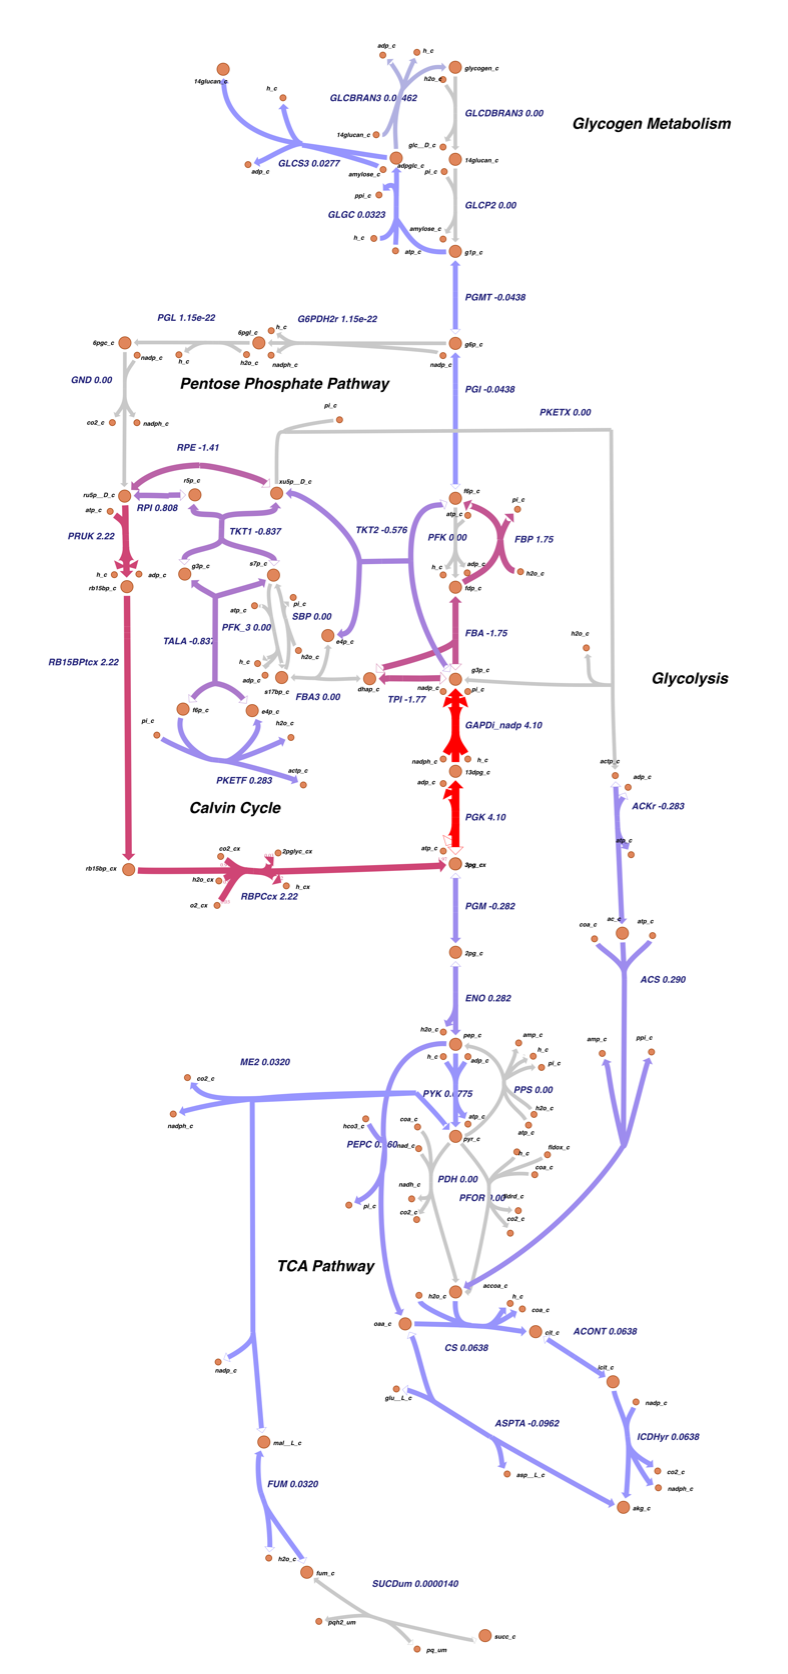
\includegraphics[width=0.6\textwidth]{images/chap8/image02.png}
    \label{fig:ch802}
\end{figure}
\FloatBarrier

\subsection{Integrating Regulation into a Model}
A cell does not just allow its reactions to occur randomly, but instead must maintain strict control over which reactions are active and which are not. Therefore, a cell regulates the expression of the genes whose products involve enzymes or other products that control the activity of these reactions. This regulation can be incorporated into a model based on some mathematical principles, primarily the derived Hill function based on the law of mass action. Since the focus of this handbook is to provide practical assistance over understanding the theory, we direct the reader to other readings for further understanding of this derivation. Ultimately, the expression of a gene is controlled by its promoter which can be bound to by a transcription factor (TF) to either turn the promoter on, thereby expressing the gene, or turn the promoter off, thereby preventing or lowering gene expression. This idea can be represented through the chemical equation $promoter+TF \leftrightarrow promoter.TF$. Therefore, based on the assumption of rapid binding for rapid equilibrium, if a transcriptional factor turns off a gene, it can be represented through the differential equation of
 $$\frac{d[Promoter.TF]}{dt}=kon[promoter][TF]-koff[promoter.TF]=0$$
If a gene is expressed, it is transcribed to become mRNA. Therefore, one can also derive the equation $$\frac{d[mRNA]}{dt}=k1[promoter.TF]$$ The previous two equations can be combined and further derived to become
$$\frac{[Protein]}{dt}=[Protein]=\frac{[TF]}{Kd+[TF]}-d2[Protein]$$ 
Kd is the amount of TF-promoter bindings required to reach half of the max amount of protein that can be produced. Notably, similar to the kinetics based model requiring data regarding enzymatic kinetics, this approach requires knowledge of the binding profile for transcriptional regulators and subsequent mRNA transcript levels \parencite{Vivek-Anath2016}. Notably, this can be found based on omics data which is growing in accessibility due to the development of high-throughput technologies.



